\section{Layer~5 – Autonomous Optimization}
\label{sec:layer5}

% ----- SUPERKRACHT -----
\begin{tcolorbox}[colback=blue!5, colframe=blue!60, title=\textbf{Superpower: The Optimiser}]
\begin{center}
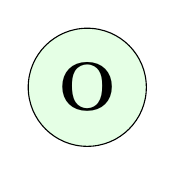
\begin{tikzpicture}
  \node[draw, circle, fill=green!10, minimum size=1.5cm, font=\bfseries\Huge] {O};
\end{tikzpicture}
\textit{“How can I get better at what I do?”}
\end{center}
\end{tcolorbox}

Pixel can now recognise groups of pixels and lay cause‑and‑effect links.
But the world does not stand still, and neither does Pixel.  Layer~5
gives Pixel the ability to \textbf{improve himself} – just like you
play a video game, die, and discover you’d better stick to the left
side of the screen.

\begin{tcolorbox}[colback=yellow!5, colframe=yellow!80, title=Real‑life analogy]
Imagine learning to juggle.  The first time the balls drop immediately.
But your brain remembers the motion, adjusts your arms a little each
time, and after a week it suddenly works.  Layer~5 does the same for
Pixel: it continuously tweaks the connections in its hypergraph so that
predictions get better and better.
\end{tcolorbox}

\textbf{Pixel’s approach.}
Pixel uses a technique mathematicians call \emph{gradient descent}.
Imagine you’re blindfolded on a hill.  You feel with your feet which
way is downhill and take a small step.  You repeat this until you
stand in the valley – the point where everything works optimally.
Pixel does the same, but with millions of parameters at once.

\subsection*{Why not just try everything?}

Pixel could randomly change things, but that would take forever.
Gradient descent provides a smart shortcut to a well‑working system.
And the best part: Pixel discovers these optimal settings completely
on its own, without any human writing a manual.

\begin{tcolorbox}[colback=orange!5, colframe=orange!60, title=\textbf{What if...?}]
What if Pixel gets stuck on a hill that isn’t the true best solution –
a so‑called local optimum?  Could it ever know there’s a much better
valley behind the next mountain?
\end{tcolorbox}